\chapter{Implementation and Testing}
\subsection{Implementation Environment}
\subsubsection{Programming Tools:}
Unity Hub \& Unity Engine were used as primary development tools for the game, where game assets, scenes, physics and animations were handled.Visual Studio Community version was employed for scripting and debugging C\# scripts. It's integrated with Unity to manage game logic, AI, and player interactions.
The Unity Asset Store leveraged for acquiring free assets, such as character models, environments, and particle effects to enrich the game's visuals and functionalities.
\subsubsection{Repository Setup \& Version Control:}
Git \& GitHub was used as a version control system to track changes and maintain backups of the project. Branching and merging were used to implement new features without affecting the main build.
\subsubsection{Integration:}
The game integrated multiple components like 3D models from the Asset Store, sound assets, and physics libraries within Unity.
Testing \& Debugging was performed through Visual Studio and Unity’s built-in play testing features.
In Unity, the Play Mode allows you to run the game within the Unity Editor itself. This lets you test the game in real time without needing to build and deploy it to a separate platform.
You can observe the game’s behavior, make changes to objects, scripts, and variables on the fly.
It helps in identifying issues such as gameplay bugs, AI behavior, and physics problems.
\subsubsection{Team Development Tools}
To make a plan and for easy management of the project, Trello was used.
\subsection{High Level Description Major Program Modules:}
The high-level program modules consist of the main classes that play a crucial role in the core functionality of the system. These key classes manage essential operations such as game logic, user interaction, and overall flow. While there are additional supporting classes that handle specific tasks (e.g., utilities, minor features), the main classes serve as the backbone of the program, driving the primary functionality and interactions within the system.
\subsection{PlayerController.cs}
\begin{itemize}
	\item \textbf{Description:} This module handles player input, movements, and interactions with the environment. 
	It defines how the character moves in response to user input and interacts with in-game objects.
	
	\item \textbf{Data Tables:} Keeps track of player stats such as health, position, inventory, and weapons.
	\item \textbf{Error Handling:} Includes checks for invalid inputs and collision detection to avoid bugs related to character movement.
\end{itemize}
\subsection{EnemyAI.cs}
\begin{itemize}
	\item \textbf{Description:} Controls enemy behavior, including patrol routes, detection of the player, and attack patterns. The enemy reacts when the player enters its detection zone.
	\item \textbf{Data Tables:} Enemy health, position, and state (idle, attack, patrol).
	\item \textbf{Error Handling:} Implements fail-safes to reset enemy states if unexpected behavior occurs, such as getting stuck in the environment.
\end{itemize}
\subsubsection{InventorySystem.cs}
\begin{itemize}
	\item \textbf{Description:} Manages the player’s inventory, including adding, removing, and using items. Links the player's interactions with the in-game shop.
	\item \textbf{Data Tables:} Item IDs, quantities, and descriptions.
	\item \textbf{Error Handling}: Prevents overflow (carrying more items than allowed) and invalid item usages.
\end{itemize}
\subsection{UIManager.cs}

\begin{itemize}
	\item \textbf{Description}: Manages the UI elements like the HUD, menus, and in-game notifications. Ensures that UI elements update dynamically during gameplay (health bars, ammo count).
	\item \textbf{Data Tables:} UI elements’ visibility, text, and buttons.
	\item \textbf{Error Handling:} Detects and fixes null references in UI elements to prevent crashes.
\end{itemize}

\subsection{ Design of Implemented Module Structure:}
Below is the diagram for Module Structure
\\
\\
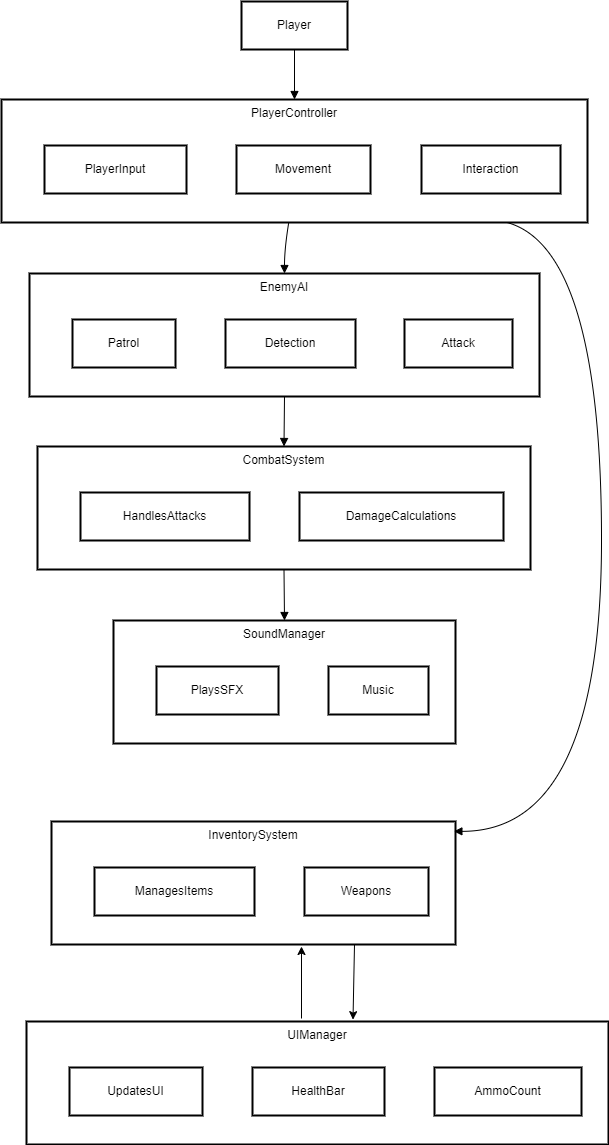
\includegraphics[width=16cm,height=18cm]{C://Users/PMLS/Desktop/Thesis/Latex Thesis/Design of Implemented Module Structure.png}
\\
\\
\textbf{PlayerController}:
\begin{itemize}
	\item Manages user input, character movement, and player interactions with the environment.
	\item Links to \texttt{InventorySystem} to update inventory when picking up or using items.
	\item Also links to \texttt{UIManager} to ensure the user interface reflects player status (e.g., health, ammo).
\end{itemize}

\textbf{InventorySystem}:
\begin{itemize}
	\item Manages items and weapons.
	\item Communicates with \texttt{UIManager} to display the correct items and quantities on the screen.
\end{itemize}

\textbf{UIManager}:
\begin{itemize}
	\item Updates the user interface dynamically based on player actions and status changes.
\end{itemize}

\textbf{EnemyAI}:
\begin{itemize}
	\item Handles enemy movement, patrol behavior, and attacks.
	\item Communicates with the \texttt{CombatSystem} to calculate and apply damage when the player and enemy interact.
\end{itemize}

\textbf{CombatSystem}:
\begin{itemize}
	\item Coordinates attack logic and damage calculations between the player and enemies.
\end{itemize}

\textbf{SoundManager}:
\begin{itemize}
	\item Plays sound effects (SFX) and music based on game events such as attacks, item pickups, or changes in player state.
	\end{itemize}
